\chapter{mROS 2-POSIXとROS 2}
\label{sec:mros2-posix}
\section{ROS 2}
ROS 2は,ROSの後継であり,ROS 2はROS 1と比べて,分散型のロボットシステムに対応している.
ROS 1では,主にUDPを使用したメッセージ型の通信を行っていたが,ROS 2では,DDSと呼ばれる通信ミドルウェアを採用しており,RTPS(Real Time Publish Subscribe)プロトコルを用いた
メッセージ型通信を行っている.これによって,個々のロボットが独立して動作するだけでなく,複数のロボットが協調して動作することが可能になった.
\section{mROS 2-POSIX}
\begin{figure}[ht]
    \centering
    \begin{minipage}{.48\textwidth}
        \centering
        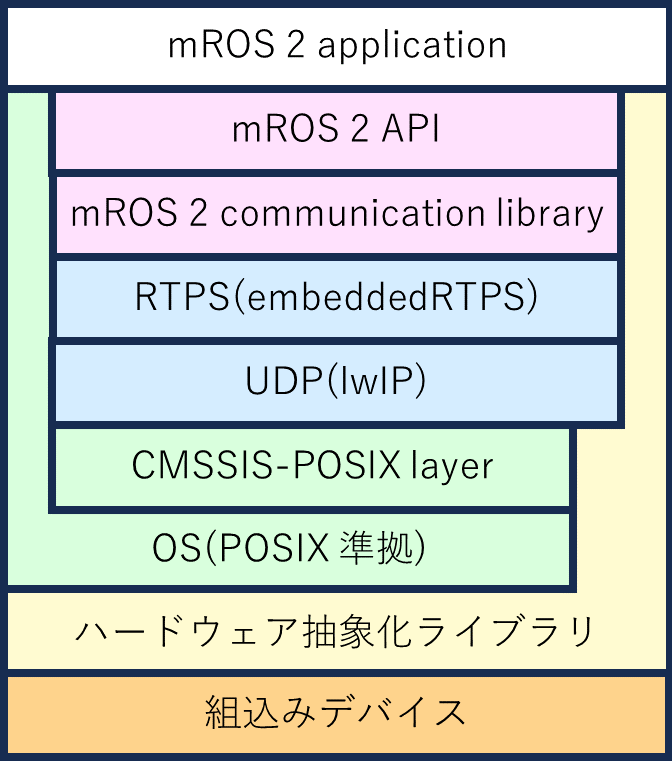
\includegraphics[width=0.9\linewidth]{images/fig1_mros2posix_a.png}
        \caption{mROS 2-POSIXの内部構成}
        \label{fig:subfig_a}
    \end{minipage}
    \hfill
    \begin{minipage}{.48\textwidth}
        \centering
        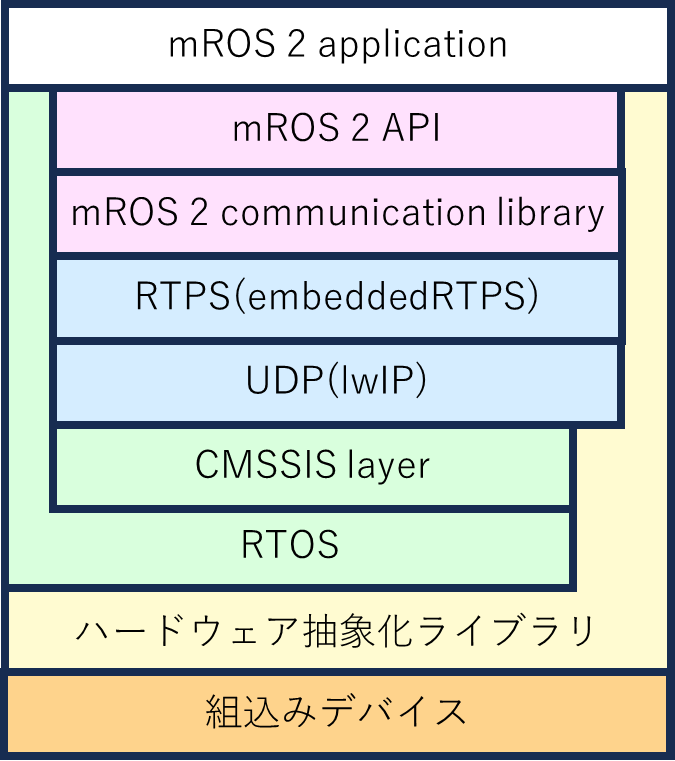
\includegraphics[width=0.9\linewidth]{images/fig1_mros2_b.png}
        \caption{mROS 2の内部構成}
        \label{fig:subfig_b}
    \end{minipage}
\end{figure}

mROS 2は,ROS 2ノードの軽量実行環境である.
このロボットソフトウェア基盤によって,分散型のロボットシステムへの組込み技術の導入ができる.
組込みデバイスは計算資源が限定的であるが,mROS 2を導入することによって組込みデバイスのリアルタイム性の向上および消費電力の削減ができる.
そして,mROS 2がPOSIX[7]に対応したのがmROS 2-POSIXである.
\\ 図1(a)は,mROS 2-POSIXのソフトウェア構成を示す.mROS 2-POSIXアプリケーション層は,ユーザが実装するROS 2ノードに相当する.
mROS 2-POSIX API層および通信ライブラリ層は,メッセージを非同期にパブリッシュやサブスクライブするためのコミュニケーションチャネルであるROS 2のTopicに相当するAPIおよび通信機能を提供する階層である.
本階層は,ROS 2のネイティブなクライアント通信ライブラリであるrclcppと互換性を保つように設計されている.
mROS 2通信ライブラリでは,rclcppのうちpub/sub通信の基本的な機能のみ実装されている.
利用可能な機能は制限されているものの,組込み技術を導入するROS 2開発者は,汎用OS向けのプログラミングスタイルを踏襲しながらC++によってmROS 2のアプリケーションを実装できる.
\\ Real Time Publish-Subscribe(以下,RTPS)プロトコルスタックにはUDPでパブリッシャとサブスクライバC++実装のembeddedRTPS[8]が採用されている.
UDPについては組込み向けのC実装であるlwIPが採用されている.
通信層のembeddedRTPSおよびlwIPはCMSAIS-POSIXに依存しており,図1(b)に示すmROS 2のCMSIS-RTOSを互換した層になっている.
最下層にはハードウェアを抽象化したライブラリがある.
\\ mROS 2-POSIXは図2に示す実行方式を採用している.
リアルタイムOSでは,組込みマイコンを実行資源の管理対象として,タスク単位でアプリケーションが実行される.
POSIXにおいてはタスクに相当する概念はプロセスであり,そこから生成されるスレッドを実行単位として処理が進行している.
しかし,mROS 2-POSIXは実行単位であるノードにPOSIXのスレッドを対応づけ,組込みマイコンでの通信処理におけるイベント割込みについては,POSIX準拠OSにおけるブロッキングAPIの発行に相当させて処理している.

